%File: formatting-instruction.tex
\documentclass[letterpaper]{article}
\usepackage{aaai}
\usepackage{times}
\usepackage{helvet}
\usepackage{courier}
\usepackage{graphicx}
\frenchspacing
\setlength{\pdfpagewidth}{8.5in}
\setlength{\pdfpageheight}{11in}
\def\mydoubleq#1{``#1''}
\def\mysingleq#1{`#1'}
\pdfinfo{
/Title ( Error Classification in OCR Historic Newspaper Archive using SVM\textsuperscript{multiclass})
/Author (Megha Gupta, Dr. Haimoti Dutta)}
\setcounter{secnumdepth}{1}  
 \begin{document}
% The file aaai.sty is the style file for AAAI Press 
% proceedings, working notes, and technical reports.
%
\title{Error Classification in OCR Historic Newspaper Archive using multi-class Support Vector Machine}

%\author{Megha Gupta\\Department of Computer Science,\\ IIIT-Delhi, India \\ meghag@iiitd.ac.in 
%\And Dr. Haimonti Dutta\\
%Center for Computational Learning Systems,\\ Columbia University, New York\\ haimonti@iiitd.ac.in}

\author{Megha Gupta and Haimonti Dutta*\\
Department of Computer Science, IIIT-Delhi\\
**Affiliated to The Center for Computational Learning Systems, Columbia University, New York\\
(meghag, haimonti)@iiitd.ac.in
}

\maketitle
\begin{abstract}
\begin{quote}
\noindent Optical Character Recognition (OCR) is a commonly used method of digitizing printed texts so that they can be searched and displayed online, stored compactly and used in text mining applications.\\
The text generated from OCR devices, however, is often garbled due to variations in quality of the input paper, size and style of the font and column layout. This adversely affects retrieval effectiveness; hence the techniques for cleaning the OCR need to be improvised. Often such techniques involve laborious and time consuming manual processing of data.\\
This paper shows the need to devise an algorithm that is scalable for a large dataset. The current state of the art algorithm used for performing multi class classification is not yet scalable. The current algorithm takes a long time to converge in a particular parameter setting.

\end{quote}
\end{abstract}

\section{Introduction}

The \textit{California Digital Newspaper Collection}\footnote{http://cdnc.ucr.edu/cgi-bin/cdnc} is an initiative of the Center for Bibliographical Studies and Research (CBSR) which is supported in part by the U.S. Institute of Museum and Library Services. It is also supported by the National Endowment for the Humanities (NEH) to digitise California newspapers for the National Digital Newspaper Program (NDNP). It contains over 400,000 pages of significant historical California newspapers published from 1846-1922.\\
OCR devices are widely used in electronic conversion of scanned images which are handwritten or printed text into a machine encoded text. The scanning generates  It finds most successful applications in the field of machine Learning, Artificial Intelligence and Pattern recognition. It deals with the problem of recognising optically generated characters be it offline or online. The performance directly depends on the quality of input document. The more constrained the input is the better will be the performance of the system. But when it comes to unconstrained handwriting, the performance is far from satisfactory. The main application areas for \cite{OCR} like Automatic number plate readers, form readers, signature verification.\\
This project deals with printed text in the form of Historical Newspaper Articles in the holdings of \cite{cdnc}. One such newspaper, The Amador Ledger published in the early 1900s by the Amador Publishing Company appealed to the community's interests by covering issues unique to gold mining. Patrons of the \cite{cdnc} continue to be interested in studying about the status of the local mining industry and consequently read the Amador Ledger on a regular basis even to this day and correct \cite{OCR} errors as they come across them.\\
In this paper, we perform error classification using Joachims multi-class Support Vector Machine algorithm called \textit{SVM\textsuperscript{multiclass}}\footnote{http://www.cs.cornell.edu/people/tj/svm\_light/svm\_multiclass.html}. We chose this algorithm as its the state of the art algorithm till now. But the experiments give altogether a different view on this algorithm. This algorithm do not converge quickly on certain parameters which are shown in table ~\ref{table: results}



%Experiments are performed on both the datasets using the same Query set. The ranked documents retrieved from both the sets are compared using a statistical measure called Spearman's Rank Order Correlation. It measures the strength of association between two ranked variables.\\
%This work can be used to determine whether the OCR text is sufficient enough to be used for the thorough text search and analysis and does it meet the user expectation without actually enhancing and enriching the text.\\


\section{Related Work}



\section{The Data}

\subsection{Log-files}
Log-files were generated using a third party software issued by \textit{Veridian}\footnote{http://www.dlconsulting.com/}, a digital library software. They used this software for logging user text corrections. Using this software, all the corrections made by the patrons were recorded in a xml format log-file. \\

\textless TextCorrectedBlock pageOID=\mydoubleq {AL19000302.1.1} blockID=\mydoubleq{P1\_TB00069} userID=\mydoubleq{[redacted]}\textgreater \\
\textless TextCorrectedLine lineID=\mydoubleq{P1\_TL00731} \textgreater \\
\textless OldTextValue\textgreater  in conjunction willi lln\&lt; Calaveras river \textless/OldTextValue\textgreater \\
\textless NewTextValue\textgreater  in conjunction with the Calaveras river \textless/NewTextValue\textgreater \\
\textless OldTextValue\textgreater  Its Eelation to the Precious \textless/OldTextValue\textgreater \\
\textless NewTextValue\textgreater  Its Relation to the Precious \textless/NewTextValue\textgreater \\
\textless OldTextValue\textgreater  ?; Metal. U \textless/OldTextValue\textgreater \\
\textless NewTextValue\textgreater  Metal. \textless/NewTextValue\textgreater \\
\textless / TextCorrectedLine \textgreater \\
\textless / TextCorrectedBlock \textgreater \\

%\begin{figure}[htbp]
%\begin{center}
%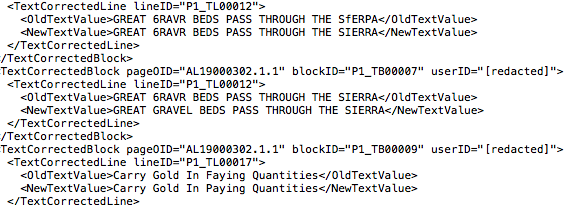
\includegraphics[width=8cm,height=3cm]{log.png}
%\caption{Log file}
%\label{fig:Logfile}
%\end{center}
%\end{figure}

The names of the log files follow a convention; the first two letters represent the initials of the newspaper followed by the date in the format yyyymmdd. For example \mydoubleq{AL19000105-changes.log} expands to Amador Ledger, 1900-01-05. There were in total 234 log files. To get an idea of the number of corrections made by user per log file, a histogram is shown in figure ~\ref{fig:histogram}

\begin{figure}[ht!]
\centering
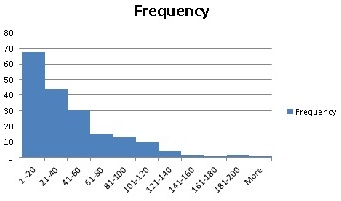
\includegraphics[width=7cm,height=5cm]{histo.jpg}
\caption{Histogram}
\label{fig:histogram}
\end{figure}

The errors rectified by the users were categorised as Spellcheck error , Addition of a new word, Capitalization error, Typo, Punctuation error. The distribution of the these classes in the dataset is shown in figure ~\ref{fig:stats}


\begin{figure}[h]
\centering
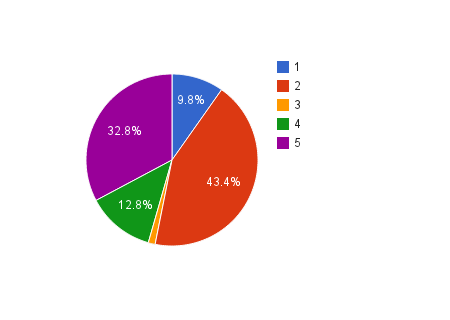
\includegraphics[width=7cm,height=5cm]{error.png}
\caption{Error Classification}
\label{fig:stats}
\end{figure}

\subsection{Newspaper}
The OCR text generated by running the OCR device on the scanned images of the newspaper was downloaded from the website using Python scripts. The general idea was to decode the names of the log files to retrieve the newspaper name and date. These were further used to formulate URLs needed to download the corresponding OCR text. For instance, \mydoubleq{AL19000105-changes.log} was converted to Amador Ledger, 1900-01-05 which was further translated to \textit{http://chroniclingamerica.loc.gov/lccn/sn93052980/1900-01-05/ed-1/seq-1/ocr.txt}.\\
Here, seq-1 refers to the first page in the sequence of pages in the newspaper. Therefore to extract issues of Amador Ledger, the only thing varied was date.
The old and its corresponding new text were stored as key value pairs of a dictionary. Once all the pairs were generated from a log file, the text in the raw corpus matching the keys of the dictionary was replaced with the value corresponding to the matched key.\\
An analysis was done to figure out the effects of noisy data on text retrieval. The experiments were run on the indexes created on both the datasets using the same query set. The documents retrieved were ranked according to the frequency of the keyword present in the document. Higher the frequency, higher the ranking order. We used Spearman correlation coefficient as the metric to measure the similarity between both our corpora. The average value of Spearman's ranked correlation coefficient calculated by our experiments was 0.625 which denotes that the association between the two corpora is not very strong but the positive value shows that if Raw OCR increases then Corrected OCR will definitely increase.\\


\section{Methodology}
%Machine Learning Algorithms and Parameters
We applied state of the art algorithm 


\section{Empirical Evaluation}

\subsection{Preprocessing \& Data Generation}

\subsubsection{Feature Construction}
Originally, there were two features in the dataset, that is old text and new text. Further features were manually crafted looking at the types of errors. In our dataset, we have six binary features consisting of sameLength, editDist\_0, editDistAbove1, editDistBelow3, editDist\_1andcaseChange, punct\_diff.
\begin{enumerate}
\item \mydoubleq{sameLength} is 1 if  both the old text and new text have same length
\item \mydoubleq{editDist\_0} is 1 if both the words are exactly same
\item \mydoubleq{editDistAbove1} is 1 if more than one edit operation is required to convert old text to new tex
\item \mydoubleq{editDistBelow3} is 1 if less than three edit operations are required to convert old text to new text
\item \mydoubleq{editDist\_1andcaseChange} is 1 if the two strings have edit distance is exactly 1 and the first character of one string change from upper case to lower case or vice versa.
\item \mydoubleq{punct\_diff} is 1 if both the old text and new text differ in any of the following punctuation marks !"\#\$\%\&'()*+,-./:;\textless=\textgreater?@[$\backslash$]\^\_`\{\textbar\}\textasciitilde
\end{enumerate}

\subsubsection{Label Construction}
The error classes were restricted to 6 classes including Spellcheck Error, Addition of a new word, Capitalization Error, Typo, Punctuation Error and No correction
These labels were assigned according to the flow graph as shown in figure
\begin{enumerate}
\item Spellcheck error : When the edit distance is between 1 and 3. For example, mounten and mountain.
\item Addition of a new word : When the edit distance is more than 3. For example, at and attend.
\item Capitalization error : When the edit distance of two strings is exactly 1 and first letter of both the strings changes from upper to lower case or vice versa. For example, largest and Largest.
\item Typo : When the edit distance is exactly one and case change is 0. For example, teh and the
\item Punctuation error : When the two strings differ by special characters contained in the set (!"\#\$\%\&'()*+,-./:;\textless=\textgreater?@[$\backslash$]\^\_`\{\textbar\}\textasciitilde). For example, 
\item No correction :  When the old and new text are same. For example, plant and plant
\end{enumerate}

The dataset was parsed to a format used by the Joachim's multi class SVM algorithm which is represented as\\
\textless target\textgreater\space\textless feature\textgreater:\textless value\textgreater ......\textless feature\textgreater:\textless value\textgreater\\
The number of rows in the dataset is 44,022. The class distribution in the dataset is shown in table ~\ref{table: classes}
\begin{table}[htdp]
\begin{center}
\begin{tabular}{l | l r |}
$ Class $ & $ no. of instances $ \\
\hline
1 & 1970 \\
\hline 
2 & 8732 \\
\hline
3 & 261 \\
\hline
4 & 2572 \\
\hline
5 & 6602 \\
\hline
6 & 23885 \\
\hline
Total & 44022 \\
\end{tabular}
\end{center}
\caption{Class Distribution}
\label{table: classes}
\end{table}


\subsection{Experiment Setup}
Experiments were performed by randomly partitioning the data into 70\% and 30\% of training and testing data respectively. For each experiment, the regularisation parameter, C and the type of kernel was varied. The experiments were performed on three machines, two of which were linux servers and the other was a dual core Mac machine with Intel Core i7 processor, 8GB RAM, 2.9 GHz of processor speed. Each experiment was iterated over different dataset for 5 times. The Average Loss and CPU runtime were noted to analyse the experiments.

\subsection{Results}

\begin{table}[htdp]
\begin{center}
\begin{tabular}{l | l | c | c | c | r | r |}
C & $AE_{L}$ & $AE_{P}$ & $AE_{R}$ & $AT_{L}$ & $AT_{P}$ & $AT_{R}$ \\
\hline
.001 & 1 & 2 & 3 & 4 & 5 & 6 \\
\hline
.01 & 1 & 2 & 3 & 4 & 5 & 6 \\
\hline
.1 & 1 & 2 & 3 & 4 & 5 & 6 \\
\hline
1 & 1 & 2 & 3 & 4 & 5 & 6 \\
\hline
10 & 1 & 2 & 3 & 4 & 5 & 6 \\
\hline
100 & 1 & 2 & 3 & 4 & 5 & 6 \\
\end{tabular}
\end{center}
\caption{Experiment Results}
\label{table: results}
\end{table}

\subsection{Discussion}



\section{Conclusion \& Future Work}




% use section* for acknowledgement
\section*{Acknowledgment}
This work is supported by funding from the National Endowment for Humanities. I would also like to express my gratitude to my Advisor, Dr. Haimonti Dutta for her support, patience and encouragement throughout the research.\\


\begin{quote}
\begin{small}
\bibliographystyle{aaai}
\bibliography{flairsPaper}
\end{small}
\end{quote}

%\nocite{datasource,cdnc,digital}
%
%\section{Bibiliography}
%\bibliography{Project_report}
%\bibliographystyle{plain}


\end{document}
